
\documentclass[a4paper,11pt]{article}
\usepackage[a4paper, margin=8em]{geometry}

% usa i pacchetti per la scrittura in italiano
\usepackage[french,italian]{babel}
\usepackage[T1]{fontenc}
\usepackage[utf8]{inputenc}
\frenchspacing 

% usa i pacchetti per la formattazione matematica
\usepackage{amsmath, amssymb, amsthm, amsfonts}

% usa altri pacchetti
\usepackage{gensymb}
\usepackage{hyperref}
\usepackage{standalone}

% imposta il titolo
\title{Appunti Calcolo Numerico}
\author{Luca Seggiani}
\date{2025}

% disegni
\usepackage{pgfplots}
\pgfplotsset{width=10cm,compat=1.9}

% imposta lo stile
% usa helvetica
\usepackage[scaled]{helvet}
% usa palatino
\usepackage{palatino}
% usa un font monospazio guardabile
\usepackage{lmodern}

% tikz in sans
\tikzset{every picture/.style={/utils/exec={\sffamily}}}

\renewcommand{\rmdefault}{ppl}
\renewcommand{\sfdefault}{phv}
\renewcommand{\ttdefault}{lmtt}

% circuiti
\usepackage{circuitikz}
\usetikzlibrary{babel}

% disponi il titolo
\makeatletter
\renewcommand{\maketitle} {
	\begin{center} 
		\begin{minipage}[t]{.8\textwidth}
			\textsf{\huge\bfseries \@title} 
		\end{minipage}%
		\begin{minipage}[t]{.2\textwidth}
			\raggedleft \vspace{-1.65em}
			\textsf{\small \@author} \vfill
			\textsf{\small \@date}
		\end{minipage}
		\par
	\end{center}

	\thispagestyle{empty}
	\pagestyle{fancy}
}
\makeatother

% disponi teoremi
\usepackage{tcolorbox}
\newtcolorbox[auto counter, number within=section]{theorem}[2][]{%
	colback=blue!10, 
	colframe=blue!40!black, 
	sharp corners=northwest,
	fonttitle=\sffamily\bfseries, 
	title=Teorema~\thetcbcounter: #2, 
	#1
}

% disponi definizioni
\newtcolorbox[auto counter, number within=section]{definition}[2][]{%
	colback=red!10,
	colframe=red!40!black,
	sharp corners=northwest,
	fonttitle=\sffamily\bfseries,
	title=Definizione~\thetcbcounter: #2,
	#1
}

% disponi problemi
\newtcolorbox[auto counter, number within=section]{problem}[2][]{%
	colback=green!10,
	colframe=green!40!black,
	sharp corners=northwest,
	fonttitle=\sffamily\bfseries,
	title=Problema~\thetcbcounter: #2,
	#1
}

% disponi codice
\usepackage{listings}
\usepackage[table]{xcolor}

\definecolor{codegreen}{rgb}{0,0.6,0}
\definecolor{codegray}{rgb}{0.5,0.5,0.5}
\definecolor{codepurple}{rgb}{0.58,0,0.82}
\definecolor{backcolour}{rgb}{0.95,0.95,0.92}

\lstdefinestyle{codestyle}{
	backgroundcolor=\color{black!5}, 
	commentstyle=\color{codegreen},
	keywordstyle=\bfseries\color{magenta},
	numberstyle=\sffamily\tiny\color{black!60},
	stringstyle=\color{green!50!black},
	basicstyle=\ttfamily\footnotesize,
	breakatwhitespace=false,         
	breaklines=true,                 
	captionpos=b,                    
	keepspaces=true,                 
	numbers=left,                    
	numbersep=5pt,                  
	showspaces=false,                
	showstringspaces=false,
	showtabs=false,                  
	tabsize=2
}

\lstdefinestyle{shellstyle}{
	backgroundcolor=\color{black!5}, 
	basicstyle=\ttfamily\footnotesize\color{black}, 
	commentstyle=\color{black}, 
	keywordstyle=\color{black},
	numberstyle=\color{black!5},
	stringstyle=\color{black}, 
	showspaces=false,
	showstringspaces=false, 
	showtabs=false, 
	tabsize=2, 
	numbers=none, 
	breaklines=true
}

\lstdefinelanguage{javascript}{
	keywords={typeof, new, true, false, catch, function, return, null, catch, switch, var, if, in, while, do, else, case, break},
	keywordstyle=\color{blue}\bfseries,
	ndkeywords={class, export, boolean, throw, implements, import, this},
	ndkeywordstyle=\color{darkgray}\bfseries,
	identifierstyle=\color{black},
	sensitive=false,
	comment=[l]{//},
	morecomment=[s]{/*}{*/},
	commentstyle=\color{purple}\ttfamily,
	stringstyle=\color{red}\ttfamily,
	morestring=[b]',
	morestring=[b]"
}

% disponi sezioni
\usepackage{titlesec}

\titleformat{\section}
{\sffamily\Large\bfseries} 
{\thesection}{1em}{} 
\titleformat{\subsection}
{\sffamily\large\bfseries}   
{\thesubsection}{1em}{} 
\titleformat{\subsubsection}
{\sffamily\normalsize\bfseries} 
{\thesubsubsection}{1em}{}

% disponi alberi
\usepackage{forest}

\forestset{
	rectstyle/.style={
		for tree={rectangle,draw,font=\large\sffamily}
	},
	roundstyle/.style={
		for tree={circle,draw,font=\large}
	}
}

% disponi algoritmi
\usepackage{algorithm}
\usepackage{algorithmic}
\makeatletter
\renewcommand{\ALG@name}{Algoritmo}
\makeatother

% disponi numeri di pagina
\usepackage{fancyhdr}
\fancyhf{} 
\fancyfoot[L]{\sffamily{\thepage}}

\makeatletter
\fancyhead[L]{\raisebox{1ex}[0pt][0pt]{\sffamily{\@title \ \@date}}} 
\fancyhead[R]{\raisebox{1ex}[0pt][0pt]{\sffamily{\@author}}}
\makeatother

\begin{document}

% sezione (data)
\section{Lezione del 02-05-25}

% stili pagina
\thispagestyle{empty}
\pagestyle{fancy}

% testo
Avevamo dato la definizione del teorema di Peano (teorema 16.2), per l'errore della generica formula di quadratura $J_n$.
Per ora quest'espressione ci risulta poco maneggevole in quanto richiede il calcolo dell'errore $G(t)$ sulla funzione $s_m(t)$, detto \textit{nucleo di Peano} (definizione 16.5).

Riprendiamo quindi la definizione dell'errore dal teorema di Peano:

$$
E_n(f) = \frac{1}{m!} \int_a^b f^{(m + 1)}(t) \cdot G(t) \, dt
$$
e accorgiamoci che se $G(t)$ non cambia segno in $[a, b]$ possiamo sfruttare il teorema della media integrale per dire che esiste un certo punto $\varepsilon \in [a, b]$ tale che:
$$
E_n(f) = \frac{1}{m!} f^{(m + 1)}(\varepsilon) \int_a^b G(t) \, dt
$$

Cerchiamo adesso di trovare una forma più maneggevole per l'integrale del nucleo di Peano $G(t)$.
Abbiamo che questa non dipende da $f$, e se valutiamo l'errore per $f(x) = x^{m + 1}$ si ottiene:
$$
E_n(x^{m + 1}) = \frac{1}{m!} \int_a^b \frac{d^{m + 1}}{dt^{m + 1}} t^{m + 1} G(t) \, dt = \frac{1}{m!} (m + 1)! \int_a^b G(t) \, dt \implies \int_a^b G(t) \, dt = \frac{E_n(x^{m + 1})}{m + 1}
$$

Prendiamo quindi questo come un \textbf{corollario} del teorema di Peano.

Osserviamo allora che se si vuole trovare una disuguaglianza del tipo:
$$
|E_n(f)| \leq M
$$
si può prendere:
$$
M = \max_{x \in [a, b]} \left| f^{(m + 1)}(x) \right| \cdot \frac{E_n(x^{m + 1})}{m + 1}
$$
dove il primo termine può essere stimato con studi di funzione o maggiorazioni esplicite, mentre il secondo termine si può calcolare esplicitamente (lo facevamo per valutare manualmente il grado di una formula di integrazione).

\subsubsection{Esempio: errore di Peano nella formula dei trapezi}
Vediamo quindi cosa si ottiene quando $n = m = 1$, cioè nel caso della formula dei trapezi.
In questo caso il nucleo è calcolato su $s_1(t)$:
$$
s_1(x - t) =
\begin{cases}
	0, \quad x < t \\
	x - t, \quad x \geq t
\end{cases}
$$
e quindi sarà:
$$
G(t) = E_n(s_m(x - t)) = \int_a^b s_1(x - t) \, dx - J_1 (s_1 (x - t))
$$

\par\smallskip

Prendiamo l'intervallo $[a, b] = [-1, 1]$ e svolgiamo i conti.
Si ha:
$$
G(t) = \int_{-1}^1 s_1(x - t) \, dx - s_1(-1 - t) - s_1(1 - t)
= \int_{-1}^1 (x - t) \, dx - 0 - 1 - t
$$
dal fatto che $-1 - t$ è sempre negativo e $1 - t$ è sempre positivo.
Proseguendo si ha:
$$
= \frac{(x - t)^2}{2} \Big|_t^1 - 1 + t = \frac{(1 - t)^2}{2} - 1 + t 
= \frac{1 + t^2 - 2t- 2 + 2t}{2} = \frac{t^2 - 1}{2} \leq 0, \quad \forall t \in [-1, 1]
$$
cioè il segno di $G(t)$ non cambia.

\par\smallskip

Questo si generalizza facilmente ad intervalli $[a, b]$ generici, in quanto con passaggi simili:
$$
G(t) = \int_a^b s_1(x - t) \, dx - J_1 ( s_1(x - t) ) = \int_t^b (x - t) \, dx - \frac{b - a}{2} s_m (a - t) - \frac{b - a}{2} s_m(b - t)
$$
da cui si ha quindi, per la definizione di $s_1(x - t)$ appena data:
$$
G(t) = \int_t^b (x - t) \, dx - \frac{b - a}{2} s_m(a - t) - \frac{b - a}{2} s_m(b - t) = \int_t^b (x - t) \, dx - \frac{b - a}{2}(b - t) 
$$
$$
= \frac{(x - t)^2}{2} \Big|^b_t - \frac{b^2 - bt - ab + at}{2} = \frac{(b - t)^2}{2} - \frac{b^2 - bt - ab + at}{2} 
$$
$$
= \frac{b^2 - 2bt + t^2 - b^2 + bt + ab - at}{2} = \frac{t^2 - bt - at}{2} = \frac{(t - a)(t - b)}{2} \leq 0, \quad \forall t \in [a, b]
$$

\noindent
\begin{minipage}{\textwidth}

Questo in realtà era chiaro osservando che il nucleo di Peano in questo caso valuta la differenza fra l'area in azzuro e la somma dell'area in azzurro e e dell'area in rosso nel seguente grafico:
\begin{center}
	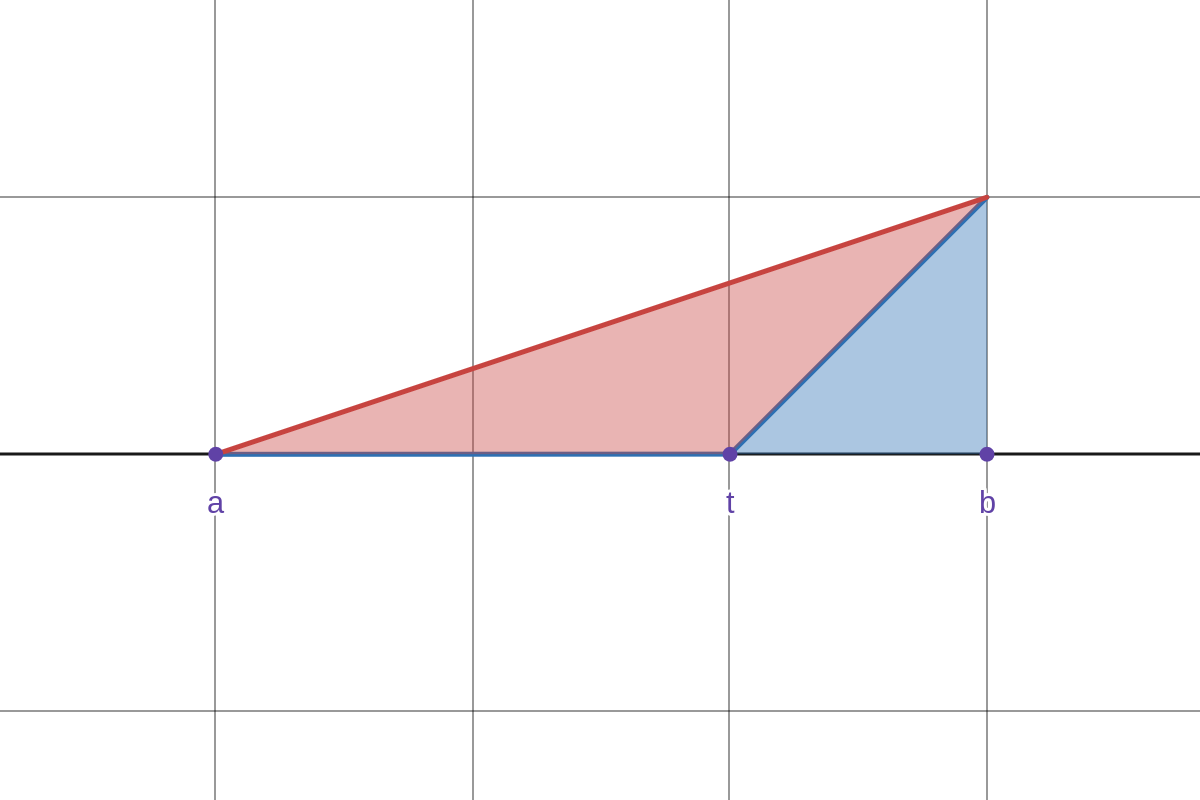
\includegraphics[scale=0.28]{../figures/peano_kernel.png}
\end{center}
che sarà chiaramente sempre $\leq 0$.

\end{minipage}

\par\smallskip

Per la formula dei trapezi vale quindi, in generale:
$$
E_1 (f) = \frac{1}{m!} f^{(m + 1)}(\varepsilon) \int_a^b G(t) \, dt = \frac{1}{m!} f^{(m + 1)}(\varepsilon) \frac{E_n(x^{m + 1})}{m + 1} = \frac{f''(\varepsilon)}{2} E_1(x^2)
$$
Preso $m = 1$.
Vediamo quindi che per $f = x^2$:
$$
E_1(x^2) = \int_a^b x^2 \, dx - \frac{b - a}{2} (a^2 + b^2) = \frac{x^3}{3} \Big|^b_a - \frac{ba^2 + b^3 - a^3 - ab^2}{2}
$$
$$
= \frac{b^3 - a^3}{3} -  \frac{ba^2 + b^3 - a^3 - ab^2}{2} = \frac{2b^3 - 2a^3 - 3ba^2 - 3b^3 + 3a^2 + 3ab^2}{6} = - \frac{(b - a)^3}{6}
$$ 
da cui:
$$
E_1(f) = - \frac{(b - a)^3}{12} \cdot f''(\varepsilon), \quad \varepsilon \in [a, b]
$$

\subsubsection{Esempio: errore di Peano nella formula di Simpson}
Si dimostra che anche la formula di Simpson è tale per cui $G(t)$ non cambia segno, quindi vale:
$$
E_2(f) = \frac{f^{(4)} (\varepsilon)}{4!} \cdot E_2(x^4) 
$$
Vediamo quindi che per l'intervallo $[-1, 1]$ vale:
$$
E_2(x^4) = \frac{2}{5} - \frac{2}{3} = - \frac{4}{15}
$$
per cui:
$$
E_2(f) = \frac{f^{(4)}(\varepsilon)}{24} \cdot \left( - \frac{4}{15} \right) = -\frac{1}{90} \cdot f^{(4)} (\varepsilon), \quad \epsilon \in [-1, 1] 
$$

Lo stesso ragionamento si può chiaramente fare per $[a, b]$ generico, cioè:
$$
E_2(x^4) = \int_{a}^{b}x^{4}dx-\frac{b-a}{6}\left(a^{4}+4\frac{\left(a+b\right)^{4}}{16}+b^{4}\right) = \frac{b^{5}-a^{5}}{5}-\frac{b-a}{24}\left(5a^{4}+4a^{3}b+6a^{2}b^{2}+4ab^{3}+5b^{4}\right)
$$
$$
= \frac{24b^{5}-24a^{5}-5\left(5a^{4}b+4a^{3}b^{2}+6a^{2}b^{3}+4ab^{4}+5b^{5}-5a^{5}-4a^{4}b-6a^{3}b^{2}-4a^{2}b^{3}-5ab^{4}\right)}{120}
$$
$$
= \frac{24b^{5}-24a^{5}-25a^{4}b-20a^{3}b^{2}-30a^{2}b^{3}-20ab^{4}-25b^{5}+25a^{5}+20a^{4}b+30a^{3}b^{2}+20a^{2}b^{3}+25ab^{4}}{120}
$$
$$
= -\frac{\left(b-a\right)^{5}}{120}
$$
da cui:
$$
E_2(f) = \frac{f^{(4)}(\varepsilon)}{24} \cdot \left( -\frac{\left(b-a\right)^{5}}{120} \right) = -\frac{(b - a)^5}{2880} \cdot f^{(4)} (\varepsilon), \quad \epsilon \in [a, b] 
$$


\subsection{Formule di quadratura interpolatorie}
Vediamo l'approccio all'approssimazione integrale che prevede scegliere $n + 1$ nodi $x_0, ..., x_n$.
In questo caso si utilizza come approssimazione di $\int_a^b f(x) \rho(x) \, dx$ la quantità:
$$
\int_a^b f(x) \rho(x) \, dx \approx \int_a^b P_n(x) \rho(x) \, dx
$$
con $P_n(x)$ polinomio di grado al più $n$ tale che:
$$
P_n(x_i) = f(x_i), \quad \forall i = 0, ..., n
$$
cioè $P_n(x)$ polinomio interpolante.

Se $f$ è sufficientemente regolare sappiamo che:
$$
f(x) = P_n(x) + R_n(x), \quad R_n(x) = \frac{\Pi (x)}{(n + 1)!} f^{(n + 1)} (\varepsilon), \quad \varepsilon \in [a, b]
$$
dal teorema 14.1.

Prendiamo quindi:
$$
\int_a^b f(x) \rho(x) \, dx = \int_a^b P_n(x) \rho(x) \, dx + \int_a^b R_n(x) \rho(x) \, dx = \int_a^b \sum_{i = 0}^n f(x_i) l_i(x) + \int_a^b R_n(x) \rho(x) \, dx
$$
dove gli $l_i(x)$ sono i polinomi della base di Lagrange:
$$
l_i(x) = \prod_{j \neq i} \frac{x - x_j}{x_i - x_j}
$$
da cui si può portare fuori la sommatoria:
$$
\int_a^b f(x) \rho(x) \, dx = \sum_{i = 0}^n f(x_i) \int_a^b l_i(x) \rho(x) \, dx + E_n(f)
$$
che ha esattamente la forma di una formula di quadratura, dove gli $f(x_i)$ sono i nodi della formula $J_n(f)$ e gli:
$$
\int_a^b l_i(x) \rho(x) \, dx
$$
a moltiplicare sono i pesi, cioè quelli che avevamo finora chiamato $a_i$.
L'errore $E_n(f)$ chiaramente si trascura.

Osserviamo che per costruzione le formule interpolatorie hanno grado di precisione almeno $n$ (chiaramente dal fatto che il polinomio interpolante di grado $n$ di un polinomio di grado $n$ è esattamente sé stesso).

Viceversa, dati $n + 1$ nodi c'è una sola formula di quadratura che ha grado di precisione $\geq n$ su qui nodi, e deve essere la formula di quadratura interpolatoria.

\subsubsection{Esempio: formule di Newton-Cotes}
L'esempio più classico delle formule di quadratura interpolatorie sono le formule di \textbf{Newton-Cotes}, che si basano sull'ipotesi di prendere nodi equispaziati su $a, b$.
Un prima scelta è riguardo all'inclusione o meno degli estremi:
\begin{itemize}
	\item Quando gli estremi $(a, b)$ sono inclusi si parla di formule di Newton-Cotes \textit{chiuse};
	\item Quando gli estremi $(a, b)$ sono esclusi si parla di formule di Newton-Cotes \textit{aperte}.
\end{itemize}

Consideriamo per adesso le formule \textbf{chiuse}, per cui:
$$
x_0 = a, \quad x_1 = h, \quad ..., \quad x_i = a + ih, \quad ..., \quad x_n = b
$$
con:
$$
h = \frac{b - a}{n}
$$
detto \textbf{passo} della formula.

I pesi $a_i$ saranno quindi:
$$
a_i = \int_a^b l_i(x) \, dx
$$

Le formule di Newton-Cotes equivalgono, per il grado 1 alle formule dei trapezi e per il grado 2 alle formule di Simosib.

Una proprietà importante delle formule di Newton-Cotes è che per ogni scelta di $n$ vale che $G(t)$ nucleo di Peano non cambia segno su $[a ,b]$, ergo si può usare la formula semplificata per l'errore di Peano:
$$
E_n(f) = \frac{f^{(m + 1)} (\varepsilon)}{(m + 1)!} \cdot E_n(x^{m + 1})
$$

Sul grado $n$ vale un fenomeno analogo al fenomeno di Runge (sezione 14.3.2).
Per $n > 7$ (cioè se si hanno più di $8$ nodi) le formule di Newton-Cotes iniziano ad avere pesi di segno alternato (mentre per $n \leq 7$ sono sempre positivi), cioè si inizia ad avere cancellazione numerica e valutare le formule diventa instabile numericamente.

\par\smallskip

Per esprimere l'errore delle formule di Newton-Cotes abbiamo quindi bisogno di trovarne l'errore $E_n(x^{m + 1})$, cioè l'errore per il monomio di grado $m + 1$ con $m$ grado di precisione.
In questo caso si assume un'espressione del tipo:
$$
E_n(f) =
\begin{cases}
	c_n \cdot h^{n + 2} \cdot f^{(n + 1)} (\varepsilon), \quad n \text{ dispari} \\			
	c_n \cdot h^{n + 3} \cdot f^{(n + 2)} (\varepsilon), \quad n \text{ pari} \\			
\end{cases}
$$

Vediamo ad esempio:
\begin{itemize}
	\item \textbf{Formula dei trapezi:} in questo caso si ha $n = 1$, $h = b - a$, da cui l'errore è esprimibile come:
		$$
		E_1 (f) = - \frac{(b - a)^3}{12} \cdot f''(\varepsilon) = -\frac{h^3}{12} \cdot f''(\varepsilon)
		$$
	\item \textbf{Formula di Simpson} in questo caso si ha $n = 2$, $h = \frac{b - a}{2}$, da cui l'errore è esprimibile come:
		$$
		E_2 (f) = - \frac{(b - a)^5}{2880} \cdot f^{(4)}(\varepsilon) = -\frac{h^5}{90} \cdot f^{(4)}(\varepsilon)
		$$
\end{itemize}

Un'altra osservazione da fare è che il grado di precisione e l'ordine della potenza di $h$ è lo stesso per una formula con grado $n$ pari e quella con grado dispari $n + 1$.
In genere, a parte il caso dei trapezi, si considerano più spesso le formule di Newton-Cotes con $n$ pari.

\par\smallskip

Vediamo nel dettaglio l'andamento del grado degli errori per qualche grado dopo lo 0.
Innanzitutto, bisogna fare una precisazione per cosa significa prendere la formula di Newton-Cotes di grado 0.
Avevamo che per formula \textit{chiusa} si intende quella che prende $n + 1$ punti estremi inclusi, mentre la formula \textit{aperta} è quella che prende $n + 1$ punti esclusi gli estremi.
Tali punti si ottengono ad esempio come:
\begin{itemize}
	\item \textbf{Formula chiusa:}
		$$
			x_i = a + i h, \quad h = \frac{b - a}{n}, \quad i = 0, 1, ..., n
		$$
	\item \textbf{Formula aperta:}
		$$
			x_i = a + (i + 1) h, \quad h = \frac{b - a}{n + 2}, \quad i = 0, 1, ..., n
		$$
\end{itemize}

Da questo risulta chiaro che sarà impossibile prendere una formula chiusa che include entrambi gli estremi quando si hanno a disposizione $n + 1 = 1$ punti per il grado $n = 0$.
Divideremo quindi fra:
\begin{itemize}
	\item \textbf{Somma di Riemann sinistra:}
		$$
			J_0^l (f) = (b - a) \cdot f(a)
		$$
	\item \textbf{Somma di Riemann destra:}
		$$
			J_0^r (f) = (b - a) \cdot f(b)
		$$
\end{itemize}

Per queste il grado è $m = 0$ e l'errore per $f = x$ risulta proporzionale al grado $2$, e non al $3$ come ci si aspetterebbe (per il punto in meno di cui non possiamo sfruttare la simmetria).
Ad esempio rispetto alla somma di Riemann sinistra si ha:
$$
E_0^l (x) = \int_a^b x \, dx - (b - a) \cdot a = \frac{b^2 - a^2}{2} - ab + a^2 = \frac{b^2 - a^2 - 2ab + 2a^2}{2} = \frac{(b - a)^2}{2}
$$

Potremo quindi considerare la formula aperta, che equivarrà alla cosiddetta \textbf{formula del punto medio}:
$$
J_0^m(f) = (b - a) \cdot f \left( \frac{a + b}{2} \right)
$$
Vediamo la particolarità che questa ha effettivamente grado $m = 1$, in quanto:
$$
E_0^m (x) = \int_a^b x \, dx - (b - a) \cdot \frac{a + b}{2} = \frac{b^2 - a^2}{2} - \frac{b^2 - a^2}{2} = 0
$$
Valutiamo quindi l'errore in $x^2$ come:
$$
E_0^m (x^2) = \frac{b^3 - a^3}{3} - (b - a) \left( \frac{a + b}{2} \right)^2 = \frac{b^3 - a^3}{3} - (b - a) \frac{a^2 + 2ab + b^2}{4}
$$
$$
= \frac{b^3 - a^3}{3} - \frac{a^2 b + 2 a b^2 b^3 - a^3 - 2 a^2 b - ab^2}{4} = \frac{b^3 - a^3}{3} + \frac{a^2 b - ab^2 - b^3 + a^3}{4}
$$
$$
= \frac{b^3 - 4a^3 + 3 a^2 b - 4 a b^2 - 3 b^3 + 3 a^3}{12} = \frac{b^3 - 3 a b^2 + 3 a^2 b - a^3}{12} = \frac{(b - a)^3}{12}
$$
cioè otteniamo un errore proporzionale a $h^3$ (lo stesso grado del metodo dei trapezi), e almeno per $x^2$ opposto a quello dato dal metodo dei trapezi.

Possiamo quindi compilare una tabella che associa i gradi di approssimazione ai gradi dell'errore per le formule di Newton-Cotes chiuse e aperte:
\begin{table}[h!]
	\center \rowcolors{2}{white}{black!10}
	\begin{tabular} { c | c | c | c | c }
		\bfseries Grado & \multicolumn{2}{c|}{\bfseries Formula} & \multicolumn{2}{c}{\bfseries Errore} \\
																		& \bfseries Aperta & \bfseries Chiusa & \bfseries Aperta & \bfseries Chiusa \\
		\hline
		0 & $2 h f_0$ & $2 h f_0$ & 3 & 2 \\ 
		1 & $\frac{3}{2} h (f_0 + f_1)$ & $\frac{1}{2} h (f_0 + f_1)$ & 3 & 3 \\
		2 & $\frac{4}{3} h (2 f_0 - f_1 + 2 f_2)$ & $\frac{1}{3} h (f_0 + 4 f_1 + f_2)$ & 5 & 5 \\
		3 & $\frac{1}{12} h (11 f_0 + f_1 + f_2 + 11 f_3)$ & $\frac{3}{8} h (f_0 + 3f_1 + 3 f_2 + f_3)$ & 5 & 5 \\
	\end{tabular}
\end{table}

\subsubsection{Esempio: formule Gaussiane}
Riprendiamo quindi anche le formule Gaussiane espresse come formule di quadratura interpolatorie.

Innanzitutto si può dire che anche per queste il nucleo di Peano $G(t)$ non cambia segno su $[a, b]$, cioè si può usare la formula di errore data dal corollario.

Un'altra proprietà è che i pesi delle formule Gaussiane sono sempre positivi, ergo non ci sono problemi di instabilità numerica per $n$ grande.

Veniamo quindi a come ricavarle.
Fissato l'intervallo $[a, b]$ e la funzione peso $\rho(x)$ si ha che le formule Gaussiane sono completamente determinate.
I nodi delle formule gaussiane si possono scrivere come zeri di particolari polinomi, detti \textit{polinomi ortogonali}.
Più precisamente sono gli zeri della successione di polinomi $\{q_n\}$, con $\deg(q_n) = n$, determinati da:
$$
< q_n, p > = 0 , \quad \forall p : \deg(p) < n
$$
sfruttando la definizione di prodotto scalare $< \cdot , \cdot >$ sullo spazio polinomiale $\mathbb{R}[x]$ data nei corsi di algebra lineare:
$$
<a, b> = \int_a^b a(x) b(x) \, dx
$$
da cui:
$$
< q_n, p > = \int_a^b q_n(x) p(x) \rho(x) \, dx
$$

\begin{itemize}
	\item
		Nel caso specifico che stavamo calcolando, con $[a, b]$ e $\rho(x) = 1$ si trova l'insieme dei \textbf{polinomi di Legendre}.
	\item 
		Usando $[a, b]$ e la funzione peso:
		$$
		\rho(x) = \frac{1}{\sqrt{1 - x^2}}
		$$
		si ottiene invece il cosiddetto \textbf{polinomio di Chebyshev di prima specie}, le cui radici sono i nodi di Chebyshev (che avevamo già incontrato nella sezione 14.3.3).
\end{itemize}

Esistono metodi ad-hoc per trovare gli zeri dei polinomi ortogonali su $[-1, 1]$. 
Una volta trovati questi si possono ottenere quelli su $[a, b]$ con il cambio di variabili:
$$
[-1, 1] \rightarrow [a, b], \quad x \rightarrow \frac{b - a}{2} x + \frac{b + a}{2}
$$
cioè una semplice operazione di scalatura lineare.

\end{document}
